\section{End-to-end Dense Video Captioning with Parallel Decoding}

\subsection{Overview}
\par Wang \textit{et al} in their paper, titled \textit{End-to-end Dense Video Captioning with Parallel Decoding} \cite{wang2021endtoend} aim to address certain issues that they identify in existing DVC work, namely, the two-stage design and handcrafted and heuristic components for event proposals generation. They model DVC as a set prediction task, and propose a model which, using a transformer architecture based on the deformable DeTR \cite{}, performs event localization and event captioning in parallel. They utilize an event counter head to predict number of events based on video understanding.

\subsection{Limitations Identified}
\par Wang \textit{et al} identify the following limitations of previous DVC work:
\subsubsection{Two-stage design} Most models use a localize-then-describe strategy for DVC tasks, i.e. they first localize the events, and then feed these events to a captioning module for generating captions. These methods usually are not trained end-to-end; rather the two stages are trained separately. Consequently, the mutual promotion of the two subtasks is limited; captioning is considered a downstream task and hence inter-task associations are not learned.

\begin{figure}[h]
\centering
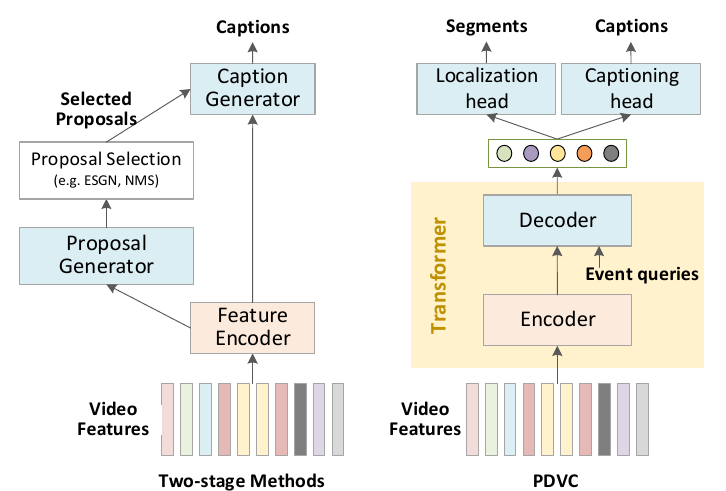
\includegraphics[width=0.5\linewidth]{assets/img/pdvc/single-stage.png}
\caption{Two-stage architecture versus proposed single-stage PDVC architecture. Image courtesy \cite{wang2021endtoend}}
\end{figure}

\subsubsection{Unreliable Event Count Estimation} The number of event proposals is often heuristically determined, for example by applying manual thresholds on confidence scores, choosing the top $k$ events, non-maximum suppression (NMS), et cetera. These methods introduce a lot of design issues, assumptions and hyperparameters, and the authors label these as \textit{hand-crafted components} \cite{wang2021endtoend}. An unreliable event count estimation can cause either missing information in captions due to under-estimation, or redundancy in captions due to over-estimation.

\subsubsection{Design of Proposal Generators} Most proposal generators use anchors and/or post-processing of events. Again, this brings in more hyperparameters and assumptions.

\subsection{Proposed Solution}

\begin{figure}
\centering
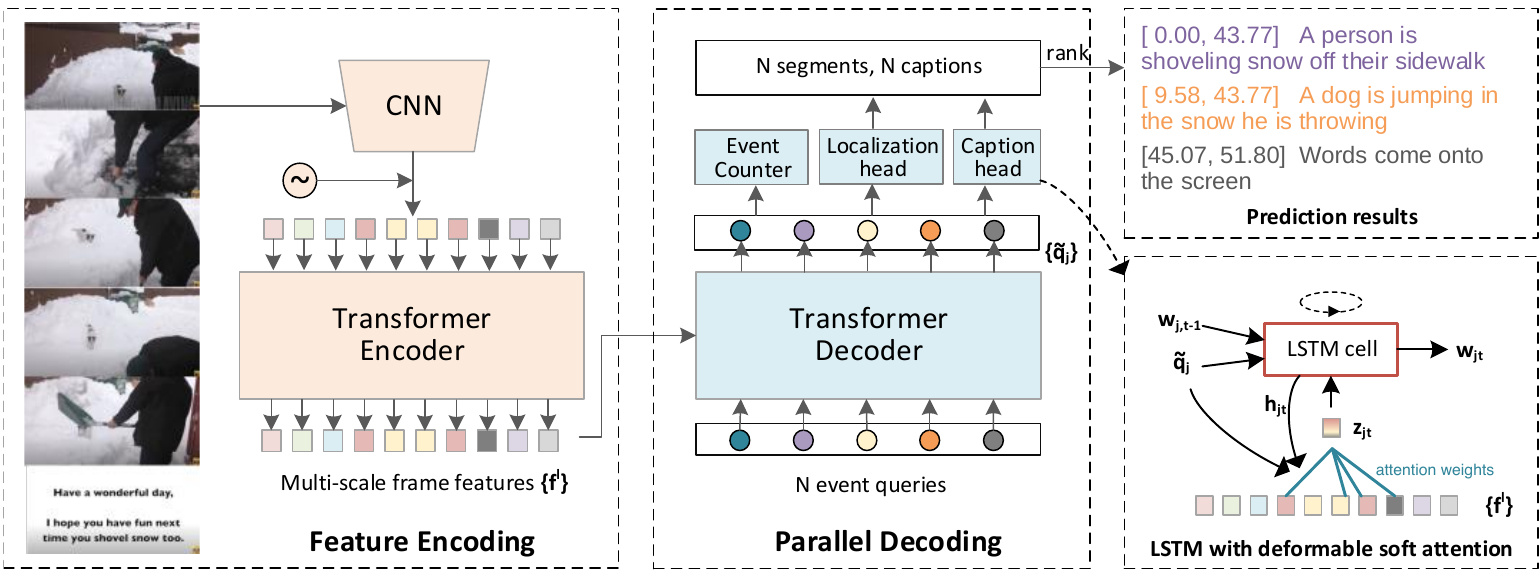
\includegraphics[width=\linewidth]{assets/img/pdvc/arch.png}
\caption{PDVC Architecture. Image courtesy \cite{wang2021endtoend}}
\end{figure}

\par Wang \textit{et al} model the task of dense video captioning as a \textit{set prediction task} \cite{wang2021endtoend}, i.e. the problem is to predict a set of $\{t_j^s, t_j^e, S_j\}$, where $t_j^s$ and $t_j^e$ are the start and end timestamps of the event $j$, and $S_j$ is its caption. 

\par This set is of size $N_{set}$, which is predicted by the \textit{event counter}. The event counter learns to predict the number of events in a video based on video understanding instead of heuristics.

\par The model performs the subtasks of event localization and caption generation in parallel, making the model a \textit{single-stage pipeline} as opposed to the majority of previous work. This enables the end-to-end training of the entire model, and performance is boosted by mutual promotion of the two tasks.

\par The authors report localization performance being at par with state-of-the-art, while captioning quality is reported to be better than state-of-the-art at the time.


\subsubsection{Feature Encoding}
The features are extracted from videos using pretrained video encoders C3D and TSN. Temporal convolutional layers are applied to get \textit{multi-scale features}, to get feature sequences across multiple resolutions \cite{wang2021endtoend}. These multi-scale features with positional encoding are given to the encoder of the deformable transformer, which uses \textit{multi-scale deformable attention} to give a context vector as output.

\subsubsection{Parallel Decoding}
\par The decoder layers of the deformable transformer, which use multi-scale deformable attention in place of cross-attention (self-attention remaining unchanged as in \cite{tfm}). The decoder layers query event-level features from the context vector conditioned on $N$ learnable embeddings (termed \textit{event queries}, $q_j$) and corresponding scalar reference point $p_j$. An event query $q_j$ serves as an initial guess of event features and $p_j$ serves as that of the center point of the event, and these are refined at each decoder layer. The output representation from decoder layers is given to the following three heads directly and in parallel.

\subsubsection{Localization Head} This head performs box prediction with a center and length offset with respect to the reference point, and performs binary classification to output the foreground confidence for each event query. Both these predictions are performed using fully connected layers. The output of this head is $\{ t_j^s, t_j^e, c_j^{loc} \}$, where $c_j^{loc}$ is the localization (foreground) confidence.

\subsubsection{Captioning Head} The authors propose two variants for the captioning head: (1) a vanilla LSTM and (2) an LSTM using deformable soft attention. The latter uses cues from the combination of caption words and the event features, while the former uses only event features.

\subsubsection{Event Counter} This head consists of a max-pooling layer to compress event queries into a global feature vector, which is fed to a fully connected layer to predict vector $r_len$, from which $N_{set}$ is found by the $argmax$ function. 

Finally, the top $N_{set}$ events from N event queries in terms of their overall confidence scores $c_j$ are selected.
$$ c_j = c_j^{loc} + \mu \frac{1}{M_j^{\gamma}} \sum_{t=1}^{M_j}{log( c^{cap}_{jt} )} $$
\par where $\mu$ is a balancing factor between localization and captioning confidence, $\gamma$ is a modulation factor to rectify the influence of caption length $M_j$.


\subsubsection{Set Prediction Loss}
\par The Hungarian algorithm is used to match predicted events with ground truths to find best bipartite matching results. The two sets are the predicted events and the ground truth events. Matching cost is defined as:
$$ C = \alpha_{giou} L_{giou} + \alpha_{cls} L_{cls} $$
\par and the set prediction loss is defined as:
$$ L = \beta_{giou} L_{giou} + \beta_{cls} L_{cls}  + \beta_{ec} L_{ec} + \beta_{cap} L_{cap}$$

\par Here $L_{giou}$ is the generalized IoU between predicted temporal segments and ground truth segments, $L_{cls}$ is the focal loss between predicted classifications score and ground truth labels, $L_{ce}$ is the cross-entropy between predicted event count distribution and ground truth and $L_{cap}$ is the cross-entropy loss between predicted word distribution and ground truth (normalized by caption length).
